\documentclass[border=12pt]{standalone}
\usepackage{amsmath,amssymb,bm}
\usepackage{tikz}
\usetikzlibrary{positioning,arrows.meta,fit,backgrounds}
\tikzset{
  box/.style={draw, rounded corners=4pt, line width=0.8pt, inner sep=7pt, align=center, fill=white},
  stage/.style={draw, rounded corners=6pt, line width=0.8pt, inner sep=8pt},
  lab/.style={font=\bfseries\large, anchor=south west},
  arr/.style={-{Stealth[length=3mm]}, line width=1pt},
  darr/.style={-{Stealth[length=3mm]}, line width=0.8pt, dashed, gray},
}
\definecolor{cbulk}{HTML}{E3EEFB}\definecolor{cshear}{HTML}{E6F5E6}
\definecolor{ccent}{HTML}{FDF0E0}\definecolor{cchart}{HTML}{F3E6F7}\definecolor{cdata}{HTML}{F2F2F2}
\definecolor{cnote}{HTML}{FFFBE0}
\newcommand{\NN}{\mathcal{N}}
\newcommand{\re}{\operatorname{Re}}\newcommand{\im}{\operatorname{Im}}
\newcommand{\gb}{\bar g}\newcommand{\eb}{\bar e}\newcommand{\Eb}{\bar E}
\newcommand{\bnd}{\operatorname{b}}

\begin{document}
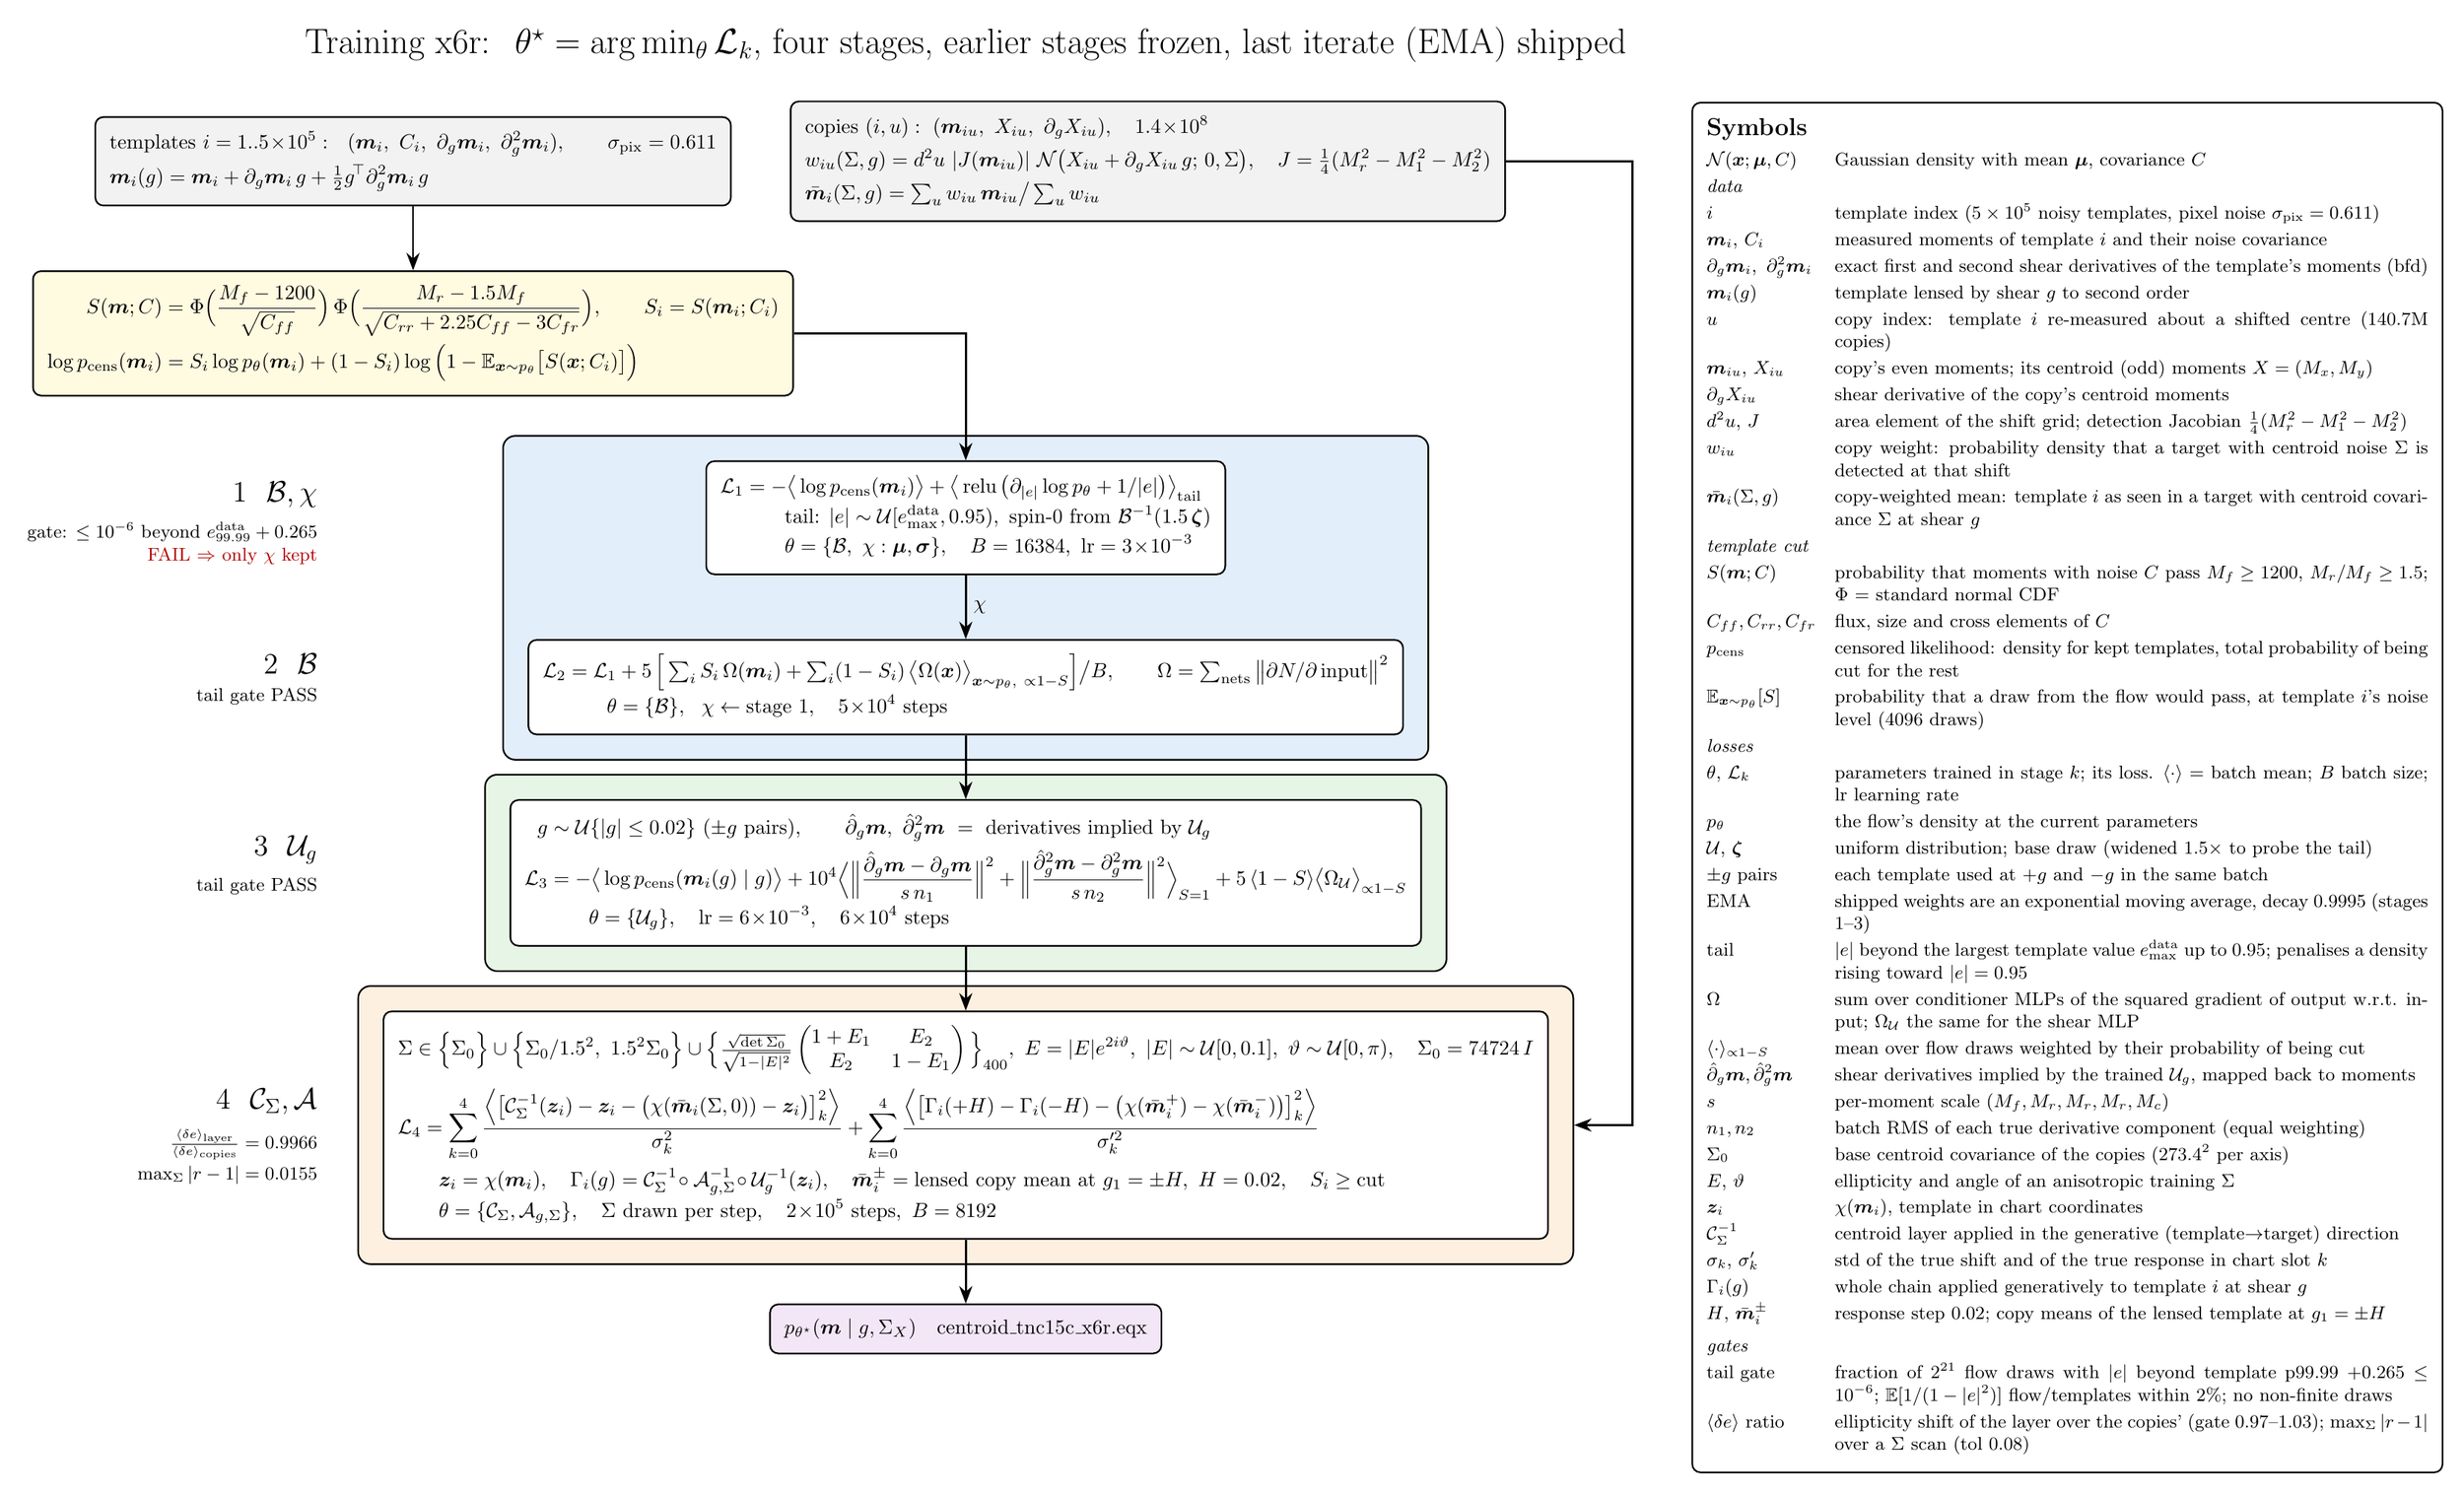
\begin{tikzpicture}[node distance=11mm]
\node[font=\LARGE] (title) {Training x6r: \ $\theta^\star=\arg\min_\theta \mathcal L_k$, four stages, earlier stages frozen, last iterate (EMA) shipped};

\node[box, fill=cdata, below=8mm of title, xshift=-95mm] (tm) {$\begin{aligned}
&\text{templates } i=1..5\!\times\!10^5:\ \ (\bm m_i,\ C_i,\ \partial_g\bm m_i,\ \partial_g^2\bm m_i),\qquad \sigma_{\text{pix}}=0.611\\
&\bm m_i(g)=\bm m_i+\partial_g\bm m_i\,g+\tfrac12 g^{\!\top}\partial_g^2\bm m_i\,g
\end{aligned}$};
\node[box, fill=cdata, right=10mm of tm] (cp) {$\begin{aligned}
&\text{copies } (i,u):\ (\bm m_{iu},\ X_{iu},\ \partial_g X_{iu}),\quad 1.4\!\times\!10^8\\
&w_{iu}(\Sigma,g)=d^2u\ |J(\bm m_{iu})|\ \NN\big(X_{iu}+\partial_gX_{iu}\,g;\,0,\Sigma\big),\quad J=\tfrac14(M_r^2-M_1^2-M_2^2)\\
&\bar{\bm m}_i(\Sigma,g)=\textstyle\sum_u w_{iu}\,\bm m_{iu}\big/\sum_u w_{iu}
\end{aligned}$};

\node[box, fill=cnote, below=of tm] (cut) {$\begin{aligned}
S(\bm m;C)&=\Phi\Big(\frac{M_f-1200}{\sqrt{C_{ff}}}\Big)\,\Phi\Big(\frac{M_r-1.5M_f}{\sqrt{C_{rr}+2.25C_{ff}-3C_{fr}}}\Big),\qquad S_i=S(\bm m_i;C_i)\\
\log p_{\text{cens}}(\bm m_i)&=S_i\log p_\theta(\bm m_i)+(1-S_i)\log\Big(1-\mathbb E_{\bm x\sim p_\theta}\big[S(\bm x;C_i)\big]\Big)
\end{aligned}$};

\node[box, below=of cut, xshift=95mm] (s1) {$\begin{aligned}
\mathcal L_1&=-\big\langle\log p_{\text{cens}}(\bm m_i)\big\rangle
+\big\langle\operatorname{relu}\big(\partial_{|e|}\log p_\theta+1/|e|\big)\big\rangle_{\text{tail}}
\\[-2pt]&\qquad\text{tail: }|e|\sim\mathcal U[e^{\text{data}}_{\max},0.95),\ \text{spin-0 from }\mathcal B^{-1}(1.5\,\bm\zeta)\\[-2pt]&\qquad\theta=\{\mathcal B,\ \chi:\bm\mu,\bm\sigma\},\quad B=16384,\ \text{lr}=3\!\times\!10^{-3}
\end{aligned}$};
\node[box, below=of s1] (s2) {$\begin{aligned}
\mathcal L_2&=\mathcal L_1+5\,\Big[\textstyle\sum_i S_i\,\Omega(\bm m_i)+\sum_i(1-S_i)\,\big\langle\Omega(\bm x)\big\rangle_{\bm x\sim p_\theta,\ \propto 1-S}\Big]\big/B,\qquad
\Omega=\sum_{\text{nets}}\big\|\partial N/\partial\,\text{input}\big\|^2\\[-2pt]
&\qquad\theta=\{\mathcal B\},\ \ \chi\leftarrow\text{stage 1},\quad 5\!\times\!10^4\ \text{steps}
\end{aligned}$};
\node[box, below=of s2] (s3) {$\begin{aligned}
g&\sim\mathcal U\{|g|\le0.02\}\ (\pm g\ \text{pairs}),\qquad \hat{\partial}_g\bm m,\ \hat{\partial}^2_g\bm m\ =\ \text{derivatives implied by }\mathcal U_g\\
\mathcal L_3&=-\big\langle\log p_{\text{cens}}(\bm m_i(g)\mid g)\big\rangle
+10^4\Big\langle\Big\|\frac{\hat\partial_g\bm m-\partial_g\bm m}{s\,n_1}\Big\|^2+\Big\|\frac{\hat\partial^2_g\bm m-\partial^2_g\bm m}{s\,n_2}\Big\|^2\Big\rangle_{S=1}
+5\,\langle 1-S\rangle\big\langle\Omega_{\mathcal U}\big\rangle_{\propto1-S}\\[-2pt]
&\qquad\theta=\{\mathcal U_g\},\quad \text{lr}=6\!\times\!10^{-3},\quad 6\!\times\!10^4\ \text{steps}
\end{aligned}$};
\node[box, below=of s3] (s4) {$\begin{aligned}
&\Sigma\in\Big\{\Sigma_0\Big\}\cup\Big\{\Sigma_0/1.5^2,\ 1.5^2\Sigma_0\Big\}\cup\Big\{\tfrac{\sqrt{\det\Sigma_0}}{\sqrt{1-|E|^2}}\begin{pmatrix}1+E_1&E_2\\E_2&1-E_1\end{pmatrix}\Big\}_{400},\ E=|E|e^{2i\vartheta},\ |E|\sim\mathcal U[0,0.1],\ \vartheta\sim\mathcal U[0,\pi),\quad
\Sigma_0=74724\,I\\[3pt]
&\mathcal L_4=\sum_{k=0}^{4}\frac{\Big\langle\big[\mathcal C_\Sigma^{-1}(\bm z_i)-\bm z_i-\big(\chi(\bar{\bm m}_i(\Sigma,0))-\bm z_i\big)\big]_k^2\Big\rangle}{\sigma_k^2}
+\sum_{k=0}^{4}\frac{\Big\langle\big[\Gamma_i(+H)-\Gamma_i(-H)-\big(\chi(\bar{\bm m}^+_i)-\chi(\bar{\bm m}^-_i)\big)\big]_k^2\Big\rangle}{\sigma'^2_k}\\
&\qquad\bm z_i=\chi(\bm m_i),\quad \Gamma_i(g)=\mathcal C_\Sigma^{-1}\!\circ\mathcal A_{g,\Sigma}^{-1}\!\circ\mathcal U_g^{-1}(\bm z_i),\quad
\bar{\bm m}^\pm_i=\text{lensed copy mean at }g_1=\pm H,\ H=0.02,\quad S_i\ge\text{cut}\\[-2pt]
&\qquad\theta=\{\mathcal C_\Sigma,\mathcal A_{g,\Sigma}\},\quad \Sigma\ \text{drawn per step},\quad 2\!\times\!10^5\ \text{steps},\ B=8192
\end{aligned}$};

\node[box, fill=cchart, below=of s4] (out) {$p_{\theta^\star}(\bm m\mid g,\Sigma_X)$\quad centroid\_tnc15c\_x6r.eqx};

\begin{scope}[on background layer]
\node[stage, fill=cbulk, fit=(s1)(s2), inner sep=12pt] (B1) {};
\node[stage, fill=cshear, fit=(s3), inner sep=12pt] (B3) {};
\node[stage, fill=ccent, fit=(s4), inner sep=12pt] (B4) {};
\end{scope}
\foreach \n/\t in {s1/{1\ \ \mathcal B,\chi}, s2/{2\ \ \mathcal B}, s3/{3\ \ \mathcal U_g}, s4/{4\ \ \mathcal C_\Sigma,\mathcal A}}
  \node[font=\Large, anchor=east] (L\n) at ([xshift=-16pt,yshift=4mm]\n.west -| B4.west) {$\t$};

\node[anchor=north east, align=right, font=\small] at (Ls1.south east) {gate: $\le10^{-6}$ beyond $e^{\text{data}}_{99.99}+0.265$\\ \textcolor{red!70!black}{FAIL $\Rightarrow$ only $\chi$ kept}};
\node[anchor=north east, align=right, font=\small] at (Ls2.south east) {tail gate PASS};
\node[anchor=north east, align=right, font=\small] at (Ls3.south east) {tail gate PASS};
\node[anchor=north east, align=right, font=\small] at (Ls4.south east) {$\frac{\langle\delta e\rangle_{\text{layer}}}{\langle\delta e\rangle_{\text{copies}}}=0.9966$\\[2pt] $\max_\Sigma|r-1|=0.0155$};

\draw[arr] (tm.south) -- (cut.north);
\draw[arr] (cut.east) -| (s1.north);
\draw[arr] (s1) -- node[right]{$\chi$} (s2); \draw[arr] (s2) -- (s3); \draw[arr] (s3) -- (s4); \draw[arr] (s4) -- (out);
\draw[arr] (cp.east) -| ([xshift=10mm]B4.east |- cp.east) |- (B4.east);


\node[box, anchor=north west, align=left, font=\small, fill=white] at ([xshift=10mm,yshift=-14mm]current bounding box.north east) {%
\renewcommand{\arraystretch}{1.18}%
\begin{tabular}{@{}l@{\quad}p{10.2cm}@{}}
\multicolumn{2}{@{}l}{\large\textbf{Symbols}}\\[2pt]
$\NN(\bm x;\bm\mu,C)$ & Gaussian density with mean $\bm\mu$, covariance $C$\\
\multicolumn{2}{@{}l}{\textit{data}}\\
$i$ & template index ($5\times10^5$ noisy templates, pixel noise $\sigma_{\text{pix}}=0.611$)\\
$\bm m_i$, $C_i$ & measured moments of template $i$ and their noise covariance\\
$\partial_g\bm m_i,\ \partial_g^2\bm m_i$ & exact first and second shear derivatives of the template's moments (bfd)\\
$\bm m_i(g)$ & template lensed by shear $g$ to second order\\
$u$ & copy index: template $i$ re-measured about a shifted centre (140.7M copies)\\
$\bm m_{iu}$, $X_{iu}$ & copy's even moments; its centroid (odd) moments $X=(M_x,M_y)$\\
$\partial_gX_{iu}$ & shear derivative of the copy's centroid moments\\
$d^2u$, $J$ & area element of the shift grid; detection Jacobian $\tfrac14(M_r^2-M_1^2-M_2^2)$\\
$w_{iu}$ & copy weight: probability density that a target with centroid noise $\Sigma$ is detected at that shift\\
$\bar{\bm m}_i(\Sigma,g)$ & copy-weighted mean: template $i$ as seen in a target with centroid covariance $\Sigma$ at shear $g$\\[3pt]
\multicolumn{2}{@{}l}{\textit{template cut}}\\
$S(\bm m;C)$ & probability that moments with noise $C$ pass $M_f\ge1200$, $M_r/M_f\ge1.5$; $\Phi$ = standard normal CDF\\
$C_{ff},C_{rr},C_{fr}$ & flux, size and cross elements of $C$\\
$p_{\text{cens}}$ & censored likelihood: density for kept templates, total probability of being cut for the rest\\
$\mathbb E_{\bm x\sim p_\theta}[S]$ & probability that a draw from the flow would pass, at template $i$'s noise level (4096 draws)\\[3pt]
\multicolumn{2}{@{}l}{\textit{losses}}\\
$\theta$, $\mathcal L_k$ & parameters trained in stage $k$; its loss. $\langle\cdot\rangle$ = batch mean; $B$ batch size; lr learning rate\\
$p_\theta$ & the flow's density at the current parameters\\
$\mathcal U$, $\bm\zeta$ & uniform distribution; base draw (widened $1.5\times$ to probe the tail)\\
$\pm g$ pairs & each template used at $+g$ and $-g$ in the same batch\\
EMA & shipped weights are an exponential moving average, decay 0.9995 (stages 1--3)\\
tail & $|e|$ beyond the largest template value $e^{\text{data}}_{\max}$ up to $0.95$; penalises a density rising toward $|e|=0.95$\\
$\Omega$ & sum over conditioner MLPs of the squared gradient of output w.r.t. input; $\Omega_{\mathcal U}$ the same for the shear MLP\\
$\langle\cdot\rangle_{\propto1-S}$ & mean over flow draws weighted by their probability of being cut\\
$\hat\partial_g\bm m,\hat\partial^2_g\bm m$ & shear derivatives implied by the trained $\mathcal U_g$, mapped back to moments\\
$s$ & per-moment scale $(M_f,M_r,M_r,M_r,M_c)$\\
$n_1,n_2$ & batch RMS of each true derivative component (equal weighting)\\
$\Sigma_0$ & base centroid covariance of the copies ($273.4^2$ per axis)\\
$E$, $\vartheta$ & ellipticity and angle of an anisotropic training $\Sigma$\\
$\bm z_i$ & $\chi(\bm m_i)$, template in chart coordinates\\
$\mathcal C_\Sigma^{-1}$ & centroid layer applied in the generative (template$\to$target) direction\\
$\sigma_k$, $\sigma'_k$ & std of the true shift and of the true response in chart slot $k$\\
$\Gamma_i(g)$ & whole chain applied generatively to template $i$ at shear $g$\\
$H$, $\bar{\bm m}^\pm_i$ & response step $0.02$; copy means of the lensed template at $g_1=\pm H$\\[3pt]
\multicolumn{2}{@{}l}{\textit{gates}}\\
tail gate & fraction of $2^{21}$ flow draws with $|e|$ beyond template p99.99 $+0.265$ $\le10^{-6}$; $\mathbb E[1/(1-|e|^2)]$ flow/templates within 2\%; no non-finite draws\\
$\langle\delta e\rangle$ ratio & ellipticity shift of the layer over the copies' (gate 0.97--1.03); $\max_\Sigma|r-1|$ over a $\Sigma$ scan (tol 0.08)\\
\end{tabular}};
\end{tikzpicture}
\end{document}
